% --- Classical text classification (ported from the retired GenAI NLP overview deck) ---
\section{Classical Text Classification}
\begin{frame}{}
    \LARGE NLP: \textbf{Classical Text Classification}
\end{frame}

\begin{frame}{Bayes' Rule -- A Quick Look}
    \textbf{Bayes' Rule:}
    \[
        P(\text{Class} \mid \text{Words}) = \frac{P(\text{Words} \mid \text{Class}) \cdot P(\text{Class})}{P(\text{Words})}
    \]
    \vspace{1em}
    \begin{itemize}
        \item Predict class (e.g., spam or not) given the words
        \item Simple, powerful tool used in Naive Bayes classifiers
        \item Helps models reason with uncertainty
    \end{itemize}
\end{frame}

\begin{frame}{Naive Bayes for Sentiment Analysis}
    \textbf{Simple, fast probabilistic model}

    \vspace{1em}
    \textbf{Assumes:}
    \begin{itemize}
        \item Words are independent given the class (a ``naive'' assumption)
    \end{itemize}

    \vspace{1em}
    \textbf{Example:}
    \begin{itemize}
        \item \texttt{"This movie is awesome"} $\rightarrow$ $P(\text{Positive})$ high
        \item \texttt{"This movie is boring"} $\rightarrow$ $P(\text{Negative})$ high
    \end{itemize}

    \vspace{1em}
    \textcolor{green}{\faCheck\enspace Works well with BoW, TF-IDF, and N-grams}
\end{frame}

\begin{frame}[allowframebreaks]{Logistic Regression for Text Classification}
    We're already familiar with probability-based classifiers, and have seen logistic regression applied in computer vision tasks.

    \vspace{1em}
    \begin{itemize}
        \item Here, logistic regression takes word features (from BoW or TF-IDF)
        \item It learns weights to predict if text belongs to a certain class, such as:
        \begin{itemize}
            \item Positive or Negative
            \item Spam or Not Spam
        \end{itemize}
        \item Outputs a probability:
        \[
            P(\text{Class} = 1 \mid \text{features}) = \sigma(w_1x_1 + w_2x_2 + \ldots + b)
        \]
        \item Words like ``awesome'' get high weights for positive class
    \end{itemize}

    \framebreak
    \textcolor{blue}{\faBullseye\enspace \textbf{Intuition:}}
    \begin{itemize}
        \item Each word contributes a ``vote'' toward a class.
        \item The model learns which words are most important for classification.
    \end{itemize}

    \framebreak
    \begin{figure}
        \centering
        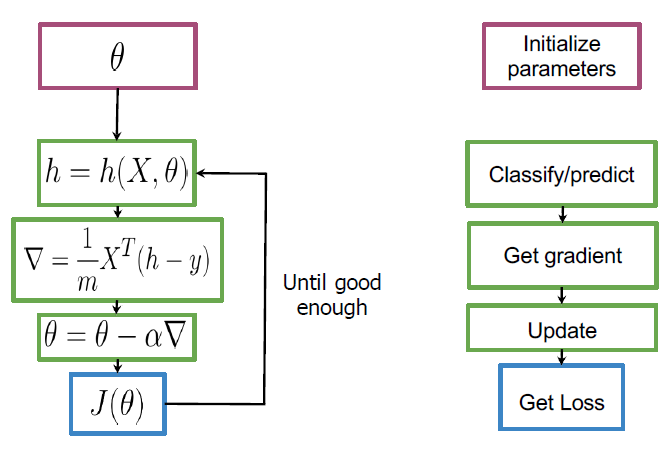
\includegraphics[height=0.67\textheight, width=\textwidth, keepaspectratio]{images/nlp/training-lr.png}
        \caption*{Training a Logistic Regression Model}
    \end{figure}
\end{frame}
